\documentclass[../p051main.tex]{subfiles}
\graphicspath{{\subfix{../figures/}}}

\begin{document}

\chapter{Magnetostatics}
\section{Current}
In our study of electrostatics, we assumed that all charges were basically stationary.
In this static equilibrium, we have $E = 0$ and a lack of net charge inside of conductors.
But in dynamic situations, charge may move more persistently!

Consider a wire with some charge flowing through it.
The rate at which charge passes through a given cross section of the wire is called the current
\[ i = \frac{dq}{dt} \]
at that point, measured in amperes (A).
To account for scenarios in which the flow of charge is not uniform over the full cross section, we can define a current density $\mbf{j}$ via
\[ i = \iint \mbf{j} \cdot d\mbf{A}, \]
where $\mbf{j}$ points in the direction of positive charge flow.
Of course we now know that it's actually negative charges (electrons) that're moving, but we stick to this convention because it isn't really hurting anyone.

Speaking of which, when we say that negative charge moves throughout a wire, we don't actually mean that electrons are rocketing through the wire at relativistic speeds, all in the same direction.
In reality their motion is much more gas-like, bouncing around with high velocities that mostly cancel each other out.
The component that does not cancel is called the drift velocity $\mbf{v}_d$, and it tends to be quite slow, on the order of one millimeter per second.
This is what creates a net movement of charge.

Now, in order to maintain this steady current throughout the wire, the electrons must be generally drifting at a constant speed.
There are two things making this happen: there is a nonzero electric field in the wire pushing the electrons along, and there is some ``drag'' force keeping the electrons from accelerating.
The forces due to these two cancel at the terminal velocity $\mbf{v}_d$.

The drift velocity is related to the current density via the equation $\mbf{j} = \rho \mbf{v}_d$, where $\rho$ is the charge density in the wire.
If we make the simplest possible assumption that the drift velocity is proportional to the electric field, we get
\[ \mbf{j} = \sigma \mbf{E}. \]
This is called Ohm's law.
Specifically, this is its intensive form since it does not depend on any of the wire's geometric properties like length or radius.
The quantity $\sigma$ is called conductivity, and it quantifies how well a material can conduct current per unit electric field.
(Its inverse $\sigma^{-1}$ is called resistivity.)

This relationship is useful, but we can use it to derive something that might be more familiar.
Suppose, now, that our wire has length $L$ and cross-sectional area $A$.
Since there is an electric field $\mbf{E}$ in the wire, there is a potential difference $\Delta V$ between the two ends; assuming constant $\mbf{E}$ and $\sigma$,
\[ \Delta V = \left| \int_{x = 0}^{x = L} \mbf{E} \cdot d\mbf{s} \right| = \left| \int_{0}^{L} \frac{j}{\sigma} dx \right| = \frac{jL}{\sigma}. \]
Since $j = i / A$, we have
\[ \Delta V = i \left( \frac{L}{\sigma A} \right) = iR, \]
where we've defined the resistance $R$, measured in ohms ($\Omega$).
This is the extensive form of Ohm's law---note that $R$ depends on the geometric properties of the wire.
Devices that are created for the purpose of providing resistance are called resistors.

\section{Circuits}
\parbox{0.65\textwidth}{
    Using wires, we can connect resistors, capacitors, and batteries (voltage sources) together to make current flow in ways that are practically useful to us.
    Schematics like the one at left are particularly useful abstractions when we want to work with circuits mathematically, like we will here.

    \vspace{6pt}
    Each circuit element is labeled with a corresponding quantity.
    The resistor has a resistance $R$, the capacitor a capacitance $C$, and the battery a voltage $V_0$.
    The battery dictates the direction of current flow---it pushes charge from low potential toward high potential, causing charge to move clockwise about the circuit.
    Right next to the battery is a switch; when closed current is allowed to flow, but when opened there is nowhere for the charge to go and the current ceases.

    \vspace{6pt}
    There are two key rules that we can exploit to ``solve'' a circuit.
}\parbox{0.35\textwidth}{
    \quad\;
    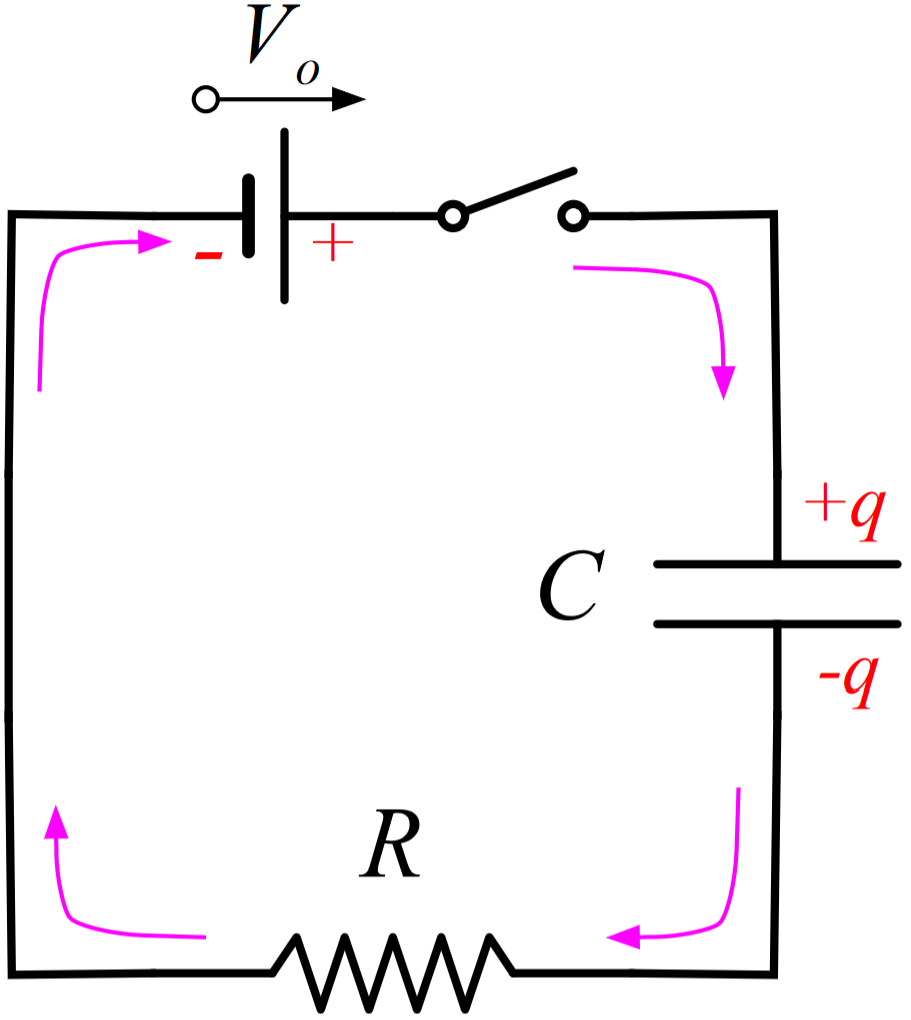
\includegraphics[width=0.3\textwidth]{rcCircuit.png}
}
\begin{itemize}
    \item By conservation of energy, the net change in potential over any loop in the circuit must be zero.
    For these purposes we can ignore any drop in potential due to travel in a wire, since it will be negligibly small compared to the potential differences across the primary circuit elements.

    \item By conservation of charge, the total current flowing into any node (any place where two wires meet) must equal the current leaving it.
\end{itemize}
Using these two rules, we are usually able to construct a system of equations that, when solved, gives the current and potential difference across each circuit element present.
We can also use them to find some convenient rules about combining like circuit elements together.
For example, we could show that pairs of resistors in parallel or in series have respective equivalent resistances
\[ R_\textrm{par} = \left( \frac{1}{R_1} + \frac{1}{R_2} \right)^{-1}, \qquad R_\textrm{ser} = R_1 + R_2. \]
We can be a bit more sophisticated, too, and examine the behavior of circuits over time.
This is especially useful in seeing, for example, how the charge on a capacitor changes while charging or discharging.

\begin{example}[Charging an RC circuit]
    Consider the above circuit.
    By conservation of energy, when the switch is closed we have
    \[ V_0 = iR + \frac{q}{C}. \]
    We can express this as a differential equation in $q(t)$, the charge on the capacitor:
    \[ \frac{dq}{dt} + \frac{1}{RC}q = \frac{V_0}{R}. \]
    With the initial condition $q(0) = 0$, the solution is
    \[ q(t) = CV_0 \left( 1 - e^{-t / RC} \right). \]
    As more charge gets deposited onto the positive plate of the capacitor, it becomes more difficult to push charge off of the other plate, around the circuit, and back onto the positive plate.
\end{example}

Finally, in order to keep the current flowing, the battery must do work on the charge to move them to higher potentials.
This work is, of course, given by $W = qV_0$, corresponding to a power
\[ P_\textrm{battery} = \frac{dW}{dt} = iV_0. \]
The resistor does an equal amount of work, so by Ohm's law we have
\[ P_\textrm{resistor} = \frac{V_0^2}{R} = i^2R \]
dissipated as heat.

\section{Magnetic Fields}
Experimental evidence has shown that electric fields do not exist in isolation.
There is another field, called the magnetic field $\mbf{B}$ (measured in teslas T), which is generated by moving charge.
If we were to ``grab'' the wire with our right hand, our thumb sticking in the direction of current, then our fingers would curl in the direction of the magnetic field.
We might verify this by looking at how the wire deflects a compass needle.

Not only are magnetic fields generated by moving charge, they also only act upon moving charge.
In particular, if a charge $q$ moves with velocity $\mbf{v}$ within a magnetic field $\mbf{B}$, then the magnetic force on the charge is
\[ \mbf{F}_B = q\mbf{v} \times \mbf{B}. \]
There are a few things to note here.
Most importantly, since $\mbf{F}_B$ is always orthogonal to $\mbf{v}$, the magnetic force can never do any work!
This perpendicularity also allows $\mbf{F}_B$ to act as a centripetal force when $\mbf{v} \perp \mbf{B}$, creating circular or helical trajectories.
Finally, if there are both electric and magnetic fields present, we add their effects to get the Lorentz force $\mbf{F} = q\mbf{E} + q\mbf{v} \times \mbf{B}$.

Npw, since magnetic fields influence moving charge, they must also influence current-carrying wires.
Suppose we have a segment of wire with current density $\mbf{j}$ and electron drift velocity $\mbf{v}_d$.
If a constant magnetic field $\mbf{B}$ acts on the wire, then the force on each electron is
\[ \mbf{F}_{B,e} = -q_e \mbf{v} \times \mbf{B} = -q_e \left( \frac{\mbf{j}}{-q_e n} \right) \times \mbf{B} = \frac{\mbf{j} \times \mbf{B}}{n}, \]
where $q_e$ is the elementary charge and $n$ is the number density of electrons.
If this segment of wire has $N$ charges, then
\[ \mbf{F}_{B,L} = N \mbf{F}_{B,e} = nAL \left( \frac{\mbf{j} \times \mbf{B}}{n} \right) = i\mbf{L} \times \mbf{B}, \]
where $L$ is the length of the segment, $A$ is its cross-sectional area, and $\mbf{L}$ points in the direction of current with magnitude $L$.

Now, everything we've done so far assumes that we already have $\mbf{B}$ at all points in space.
If we are instead only given a charge distribution, then we can find the magnetic field using the Biot-Savart law:
\[ d\mbf{B} = \frac{\mu_0}{4\pi} \frac{i d\mbf{l} \times \hat r}{r^2}, \]
where $i$ is the current in a small segment $d\mbf{l}$ of wire and $\mbf{r}$ points from the wire segment to the field point.
$\mu_0$ is called the permeability of free space.
As we'll see now, applying the Biot-Savart law is very similar to calculating electric fields via direct integration.

\begin{example}[Magnetic field due to a current-carrying ring]
    Consider a ring of wire with radius $R$ and current $i$, which flows counterclockwise when viewed from above.
    We'll determine the magnetic field at a distance $z$ above the center of the ring.

    By the right-hand rule, chunks of wire that are opposite each other on the ring create a net magnetic field that points only in the vertical direction.
    This means we can focus solely on the magnetic field's $\hat z$ component:
    \[ dB_z = |d\mbf{B}| \cos \theta = |d\mbf{B}| \frac{R}{\sqrt{R^2 + z^2}}, \]
    where $\theta$ is the angle of inclination when $z$ is viewed from a point on the ring.
    (This is equivalent to the angle each $d\mbf{B}$ makes with the vertical.)
    By the Biot-Savart law we have
    \[ |d\mbf{B}| = \frac{\mu_0}{4\pi} \left| \frac{i d\mbf{l} \times \hat r}{r^2} \right| = \frac{\mu_0 i }{4\pi r^2} |d\mbf{l} \times \hat r| = \frac{\mu_0 i}{4\pi r^2} dl. \]
    Integrating $dB_z$ to determine the total field:
    \begin{align*}
        \mbf{B}_\textrm{ring} &= \int_\textrm{ring} \frac{\mu_0 i \,dl}{4\pi (R^2 + z^2)} \frac{R}{(R^2 + z^2)^{1/2}} \hat{z} = \frac{\mu_0 i R}{4\pi (R^2 + z^2)^{3/2}} \hat{z} \int_\textrm{ring} dl = \frac{\mu_0 i \pi R^2}{2\pi (R^2 + z^2)^{3/2}} \hat{z}.
    \end{align*}
\end{example}

% We could use this result to find the magnetic field due to an infinite, densely-wrapped coil of current-carrying wire.
% In particular, if this coil (or solenoid) has radius $R$ and $n$ windings per unit length, then the magnetic field at the center is
% \[ \mbf{B}_\textrm{solenoid} = \mu_0 ni \,\hat z. \] % TODO: does this become relevant later?

This current-carrying ring will actually become our model for a magnetic dipole.
Just as we had the electric dipole moment $qd$, we have the magnetic dipole moment $iA$ where $A$ is the area enclosed by the ring.
We can see that the magnetic field due to such a dipole obeys $B \propto iA / r^3$ for $r \gg R$, just like we saw with electric dipoles (in which case it was $E \propto qd / r^3$).

\section{Ampere's Law}
Just like with electric fields, this direct integration can get a little unwieldy.
There's a cleaner way to determine magnetic fields in high-symmetry scenarios, but it'll be a bit different from Gauss's law.
The main thing is that we have never detected any magnetic monopoles.
This isn't a fundamental law of the universe or anything, it's just that every magnet we've encountered has had both a north pole and a south pole.
Thus
\[ \oiint_S \mbf{B} \cdot d\mbf{A} = 0, \qquad \nabla \cdot \mbf{B} = 0. \]
Not very helpful for our purposes.
But note that static magnetic fields are known for their twisty behavior about moving charges rather than the electric field's outward spray around point charges.
So we can instead write down Ampere's law,
\[ \oint_C \mbf{B} \cdot d\mbf{l} = \mu_0 i_\textrm{enc}, \]
where $i_\textrm{enc}$ is the net current puncturing an area enclosed by $C$.
Once again, this statement holds for all scenarios involving magnetic fields, but it's only useful in a select few with the proper symmetries.

\begin{example}[Magnetic field due to a solenoid]
    Consider an infinite coil (or solenoid) of wire with radius $R$, current $i$, and $n$ loops per unit length.
    We'll determine the magnetic field at some distance $r$ from the central axis of the solenoid.

    Let $\hat z$ represent the direction in which the magnetic field points, in accordance with the Biot-Savart law.
    The solenoid exhibits symmetry with respect to the cylindrical coordinates $\phi$ and $z$, so the magnetic field is only a function of $r$.
    Thus $\mbf{B} = B(r) \,\hat z$.

    Choose, as our Amperian loop, a length-$r$ rectangle whose height $h$ coincides with the solenoid's central axis.
    The loop is oriented such that it is parallel to $\hat z$ on the inside of the solenoid and antiparallel to $\hat z$ on the outside.

    There are two regions to consider.
    For $r < R$, we have $i_\textrm{enc} = 0$.
    Also, since the lengths of the Amperian loop are orthogonal to the magnetic field, only the heights are relevant:
    \begin{align*}
        \oint_C \mbf{B} \cdot d\mbf{l} &= \int_\textrm{up} B(0) \,\hat z \cdot dl \,\hat z + \int_\textrm{down} B(r) \,\hat z \cdot dl (-\hat z) \\
        \intertext{Now, it can be shown by a direct integration of $\mbf{B}_\textrm{ring}$ that the magnetic field at the center of an infinite solenoid is $\mbf{B}(0) = \mu_0 ni$. Thus by Ampere's law}
        0 &= \mu_0 ni h - B(r) h \;\implies\; \mbf{B}_\textrm{in}(r) = \mu_0 ni \,\hat z.
    \end{align*}
    So the magnetic field inside of a solenoid is constant.
    For $r > R$ the setup is the same, only now we have $i_\textrm{enc} = nhi$.
    ($i_\textrm{enc}$ is positive here due to how we've oriented our Amperian loop.)
    Thus by Ampere's law,
    \[ \mu_0 nih - B(r)h = \mu_0 nhi \;\implies\; \mbf{B}_\textrm{out}(r) = \mbf{0}. \]
\end{example}

\section{Frames of Reference}
At this point we have developed a complete theory of statics.
Everything we've done so far can be derived from Maxwell's time-independent equations in their integral and differential forms:
\begin{align*}
    \oiint \mbf{E} \cdot d\mbf{A} &= \frac{q}{\epsilon_0} & \nabla \cdot \mbf{E} &= \frac{\rho}{\epsilon_0} \\
    \oint \mbf{E} \cdot d\mbf{l} &= 0 & \nabla \times \mbf{E} &= \mbf{0} \\
    \oiint \mbf{B} \cdot d\mbf{A} &= 0 & \nabla \cdot \mbf{B} &= 0 \\
    \oint \mbf{B} \cdot d\mbf{l} &= \mu_0 & \nabla \times \mbf{B} &= \mu_0 \,\mbf{j}
\end{align*}
There is more to the theory of electromagnetism---we'll soon examine what happens when $\mbf{E}$ and $\mbf{B}$ are allowed to vary with time---but first we'll take a closer look at how these two fields are related, and why we so often see them lumped together as a unified electromagnetic field.

Consider the scenario illustrated below, on the left.
In a neutral wire with cross-sectional area $A$ electrons are free to move with drift velocity $\mbf{v}$, generating a current density $\mbf{j}$ in the opposite direction.
We could use Ampere's law to show that the magnetic field due to this wire is $B = \mu_0 jA / 2\pi r$, with direction determined by the right-hand rule.

Outside of the wire there is an electron that also has velocity $\mbf{v}$.
The force on this electron is purely magnetic in nature; specifically, taking the standard $x$-$y$ coordinate system,
\[ \mbf{F}_B = -q_e \mbf{v} \times \mbf{B} = q_e v \left( \frac{\mu_0 jA}{2\pi r} \right) (-\hat{\mbf{y}}) = \frac{q_e v^2 \mu_0 \rho_- A}{2\pi r} (-\hat{\mbf{y}}), \]
where we've defined the density of negative charge $\rho_-$, a positive quantity, for later convenience.
Let us call this scenario the $S$ frame.

\begin{center}
    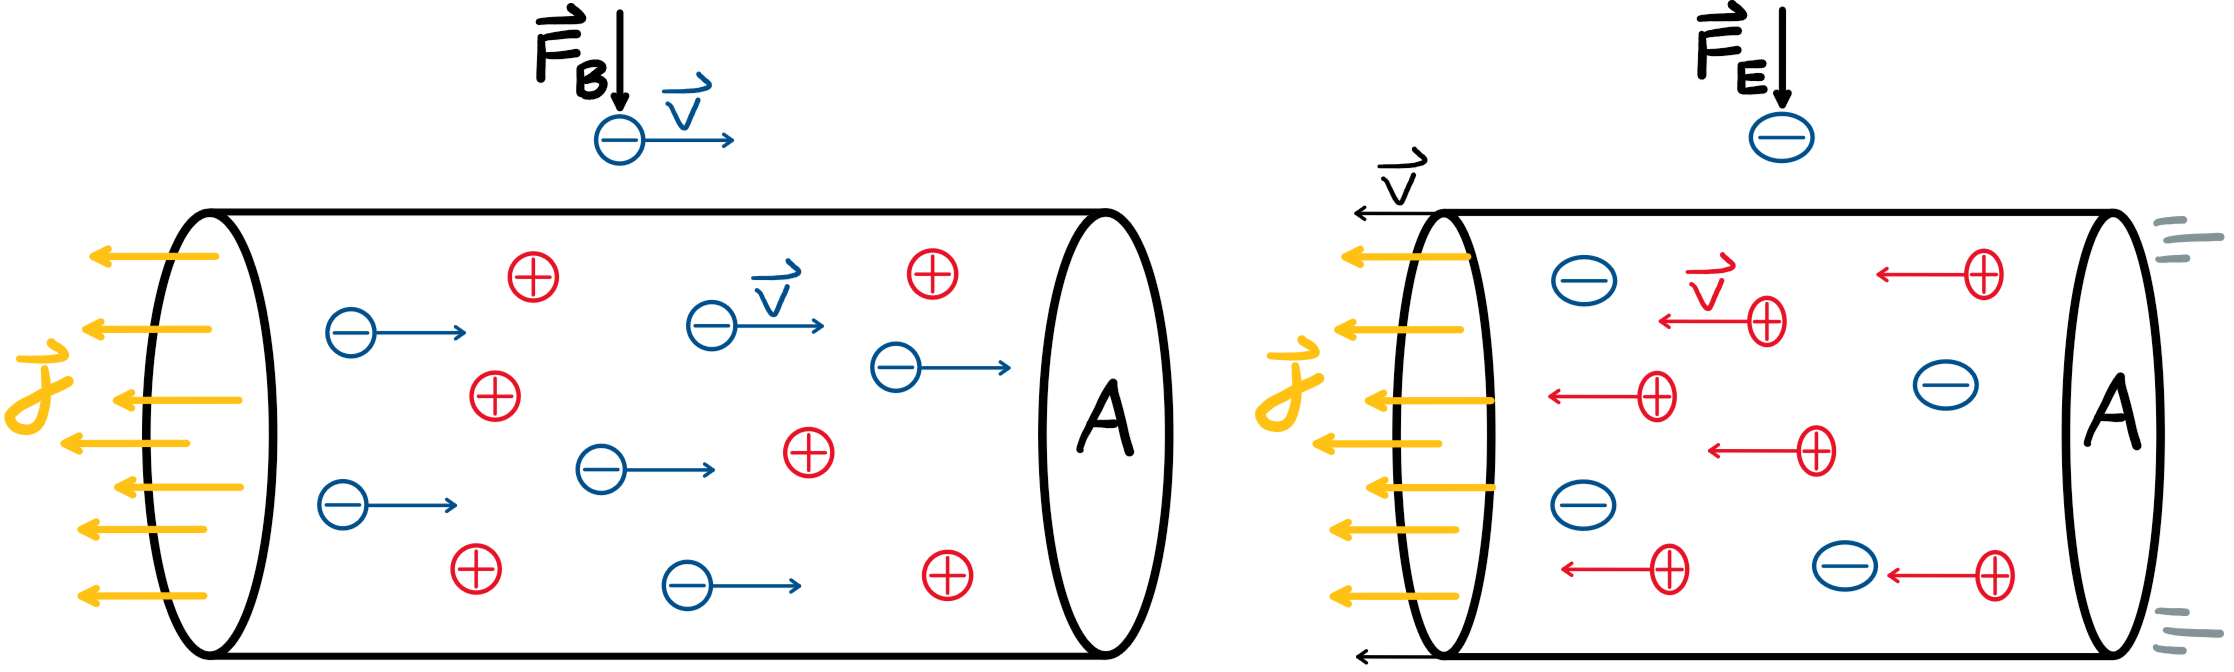
\includegraphics[width=0.9\textwidth]{wireFrames.png}
\end{center}

Now suppose we, the observer, started walking with velocity $\mbf{v}$.
We now observe the electrons to be (in net) at rest, and it is the positive charges that are actually moving.
Reason dictates that the isolated electron should still experience the same downward force, but this force cannot be magnetic since it's no longer in motion.
We must therefore uncover some sort of hidden electric force in this new $S'$ frame.

Special relativity, specifically length contraction, provides an answer!
When compared to the $S$ frame, in the $S'$ frame the positive charges are contracted while the electrons are uncontracted.
So while in the unprimed frame we had $\rho_\textrm{net} = \rho_+ - \rho_- = 0$, in the primed frame we see
\[ \rho_\textrm{net}' = \rho_+' - \rho_-' = \gamma \rho_+ - \gamma^{-1} \rho_- = \gamma \frac{v^2}{c^2} \rho_-, \]
where $\gamma$ is the Lorentz factor $\left( 1 - v^2 / c^2 \right)^{-1 / 2}$.
So the lone electron will at least experience an attractive force, which is promising.
To find its magnitude we appeal to Gauss's law: a Gaussian cylinder with radius $r'$ and length $l'$ encloses a charge $\rho' A' l' / \epsilon_0$ which generates a flux $E'(2\pi rl')$, meaning
\[ E' = \frac{\rho' A'}{2\pi \epsilon_0 r'} = \gamma \frac{v^2 \rho_- A}{2\pi \epsilon_0 c^2 r} \;\implies\; \mbf{F}_E' = \gamma \frac{q_e v^2 \rho_- A}{2\pi \epsilon_0 c^2 r} (-\hat{\mbf{y}}). \]
Now we can compare the two forces.
We could use time dilation to argue that $\mbf{F}_E = \gamma^{-1} \mbf{F}_E'$, so we have
\[ \mbf{F}_B = \mu_0 \frac{q_e v^2 \rho_- A}{2\pi r} (-\hat{\mbf{y}}), \qquad \mbf{F}_E = \frac{1}{\epsilon_0 c^2} \frac{q_e v^2 \rho_- A}{2\pi r} (-\hat{\mbf{y}}). \]
We can see that these expressions are equivalent if $\epsilon_0 \mu_0 = 1 / c^2$ and, remarkably, experimental evidence suggests that this is actually the case!
Thus a force that appeared as purely magnetic in the $S$ frame is actually purely electric in the $S'$ frame.

So it doesn't really make sense to speak about electric and magnetic fields as two separate entities.
They are, in fact, two facets of a more fundamental electromagnetic field, related to each other via a Lorentz transformation:
\begin{align*}
    \mbf{E}_{||}' &= \mbf{E}_{||} \\
    \mbf{E}_\perp' &= \gamma \left( \mbf{E}_\perp + \mbf{v} \times \mbf{B} \right) \\
    \mbf{B}_{||}' &= \mbf{B}_{||} \\
    \mbf{B}_\perp' &= \gamma \left( \mbf{B}_\perp - \frac{1}{c^2} \mbf{v} \times \mbf{E} \right)
\end{align*}
Visually, at relativistic frame velocities the electric and magnetic fields get compressed along the direction of motion, similar to how lengths are contracted at these speeds.

\end{document}